% chapter3_3.tex -- de (German)
% installation of Hifiberry MiniAmp
\section{HifiBerry {\miniamp} einrichten}
Die Community ist sich uneins dar�ber, wie hochwertig die Audioqualit�t
einer {\Bezeichnung} sein sollte. Meine pers�nliche Meinung ist, dass
gerade Kinder noch ein wesentlich besseres Geh�r haben als wir
Erwachsenen, sowohl hinsichtlich des Frequenzspektrums bei Hocht�nen als
auch bei der Empfindlichkeit. Daher sollten mal 10 Euro Mehrausgaben f�r
die Kleinen nicht \textbf{das} Entscheidungskriterium sein. Die Freude
bei Gro� und Klein wird sich bei einer qualitativ guten Umsetzung
l�nger halten. Allerdings gibt es auch Gr�nde, gerade f�r noch recht
kleine Kinder etwas leichtgewichtigere Komponenten in Form kleinerer
Lautsprecher zu verwenden.\\
So ist auch der {\miniamp} zusammen mit den verwendeten 8cm
Visaton-Laut\-spre\-chern (siehe St�ckliste in Tabelle \ref{tab:bom})
weit weg von HiFi-technischem \textit{high end}, aber in meinen Augen
ein guter Kompromiss.
%Ein echtes \textit{no-go} ist allerdings die Verwendung der
%Audiosignale aus der Ori\-gi\-nal-Klin\-ken\-buch\-se des \RPi.

Der {\miniamp} muss in \os{Raspbian} bekanntgegeben und konfiguriert
werden. Dazu sind Anpassungen in zwei Dateien erforderlich:

\textbf{\filenam{/boot/config.txt} anpassen}\\
\cmdPi{sudo nano /boot/config.txt}\\
\editor{\# Enable audio (loads snd\_bcm2835)\\
        \#\#dtparam=audio=on\comment{Diese Zeile auskommentieren!}\\
        dtoverlay=hifiberry-dac
       }

\textbf{\filenam{/etc/asound.conf} anpassen}\\
\cmdPi{sudo nano /etc/asound.conf}\\
\editor{pcm.hifiberryMiniAmp \{\\
        \textcolor{white}{\ \ \ \ }type softvol\\
        \textcolor{white}{\ \ \ \ }slave.pcm "plughw:0"\\
        \textcolor{white}{\ \ \ \ }control.name "Master"\\
        \textcolor{white}{\ \ \ \ }control.card 0\\
        \}\\
        pcm.!default \{\\
        \textcolor{white}{\ \ \ \ }type plug\\
        \textcolor{white}{\ \ \ \ }slave.pcm "hifiberryMiniAmp"\\
        \}
       }

Nach �nderungen an \filenam{/boot/config.txt} muss der {\RPi} neu
gebootet werden, damit die dort vorgenommenen �nderungen greifen:\\
\cmdPi{sudo reboot}\\
\cmdPC{ssh pi@phoniebox1}\comment{�ber \software{ssh} neu auf dem {RPi} anmelden}

Anschlie�end kann die Audioausgabe �ber den {\miniamp} �berpr�ft
werden:\\
\cmdPi{aplay -l}\comment{sollte folgende Ausgabe liefern:}\\
\stdout{**** List of PLAYBACK Hardware Devices ****\\
        card 0: sndrpihifiberry [snd\_rpi\_hifiberry\_dac], device 0: HifiBerry DAC HiFi pcm5102a-hifi-0 [HifiBerry DAC HiFi pcm5102a-hifi-0]\\
          Subdevices: 1/1\\
          Subdevice \#0: subdevice \#0}
          
Mit dem folgenden Kommando sollte an beiden Lautsprechern abwechselnd
ein sogenanntes \textit{Rosa Rauschen} ert�nen. Dieser Test kann durch
die Tastatureingabe \keyboard{Ctrl-C} unterbrochen werden:\\
\cmdPi{speaker-test -D hifiberryMiniAmp -c 2}\\
\stdout{speaker-test 1.1.8\\
        \\
        Playback device is hifiberryMiniAmp\\
        Stream parameters are 48000Hz, S16\_LE, 2 channels\\
        Using 16 octaves of pink noise\\
        Rate set to 48000Hz (requested 48000Hz)\\
        Buffer size range from 128 to 131072\\
        Period size range from 64 to 65536\\
        Using max buffer size 131072\\
        Periods = 4\\
        was set period\_size = 32768\\
        was set buffer\_size = 131072\\
        \ 0 - Front Left\\
        \ 1 - Front Right\\
        Time per period = 2.754591\\
        \ 0 - Front Left\\
        \ 1 - Front Right
       }

\cmdPi{alsamixer}\comment{Einstellung der Lautst�rke}

\begin{figure}[h]
\centering
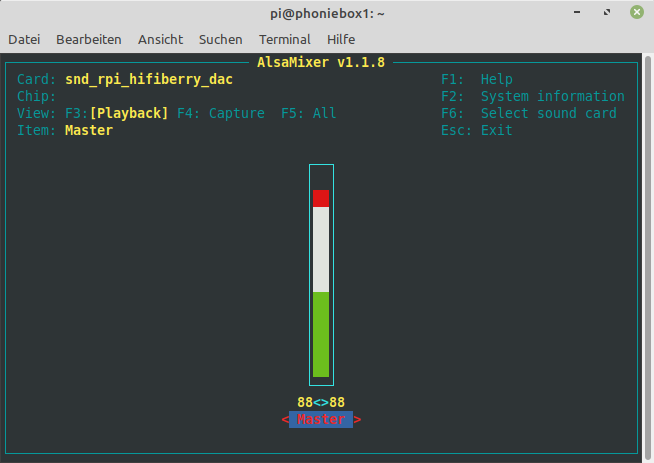
\includegraphics[width=0.9\textwidth]{software/alsamixer.png}
\caption{Lautst�rkeeinstellung mit dem \software{alsamixer}}
\label{fig:alsamixer}
\end{figure}
